\documentclass[mathserif]{beamer}

%\usetheme{LCOM}
\usetheme{Madrid}
\usepackage{hyperref}
\usepackage{listings}
\usepackage{graphicx}
\usepackage[english]{babel}
\usepackage[utf8]{inputenc}
\usepackage[T1]{fontenc}
\usepackage{booktabs}
\usepackage{amsmath,amssymb,amsthm,mathrsfs,amsfonts,dsfont}
\usepackage{adjustbox}
\usepackage{array}
\usepackage{longtable}
\usepackage{psfrag}
\usepackage{caption}
\usepackage{placeins}
\usepackage{subfig}
\usepackage{multirow}

\newcommand{\wait}{\vfill}
%\newcommand{\wait}{\pause}
	
\DeclareMathAlphabet\mathbfcal{OMS}{cmsy}{b}{n}
\newcommand\blfootnote[1]{%
	\begingroup
	\renewcommand\thefootnote{}\footnote{#1}%
	\addtocounter{footnote}{-1}%
	\endgroup
}

\setbeamertemplate{frametitle continuation}[from second][]

\title[NB hybrid PLC/Wireless transceiver prototype]{A Prototype of a Narrowband Hybrid PLC/Wireless Transceiver} 
\author[Vinícius Lagrota]{Autor: Vinícius Lagrota Rodrigues da Costa\\
	Orientador: Moisés Vidal Ribeiro}
\institute[UFJF]{Programa de Pós-Graduação em Engenharia Elétrica\\
	Universidade Federal de Juiz de Fora}
\date{15 de dezembro 2017}

\begin{document}

\begin{frame}
\maketitle 
\end{frame}

\begin{frame}
\frametitle{Outlines}
\small
\tableofcontents
\end{frame}

%------------------------------------------------------------------------------------
\section{Introduction}
%------------------------------------------------------------------------------------
\subsection{Motivation}
%%-----------------------------------------------
\begin{frame}
	\frametitle{Introduction}
	\framesubtitle{Motivation}

	\small
	\begin{itemize}		
		\item There is a recent interest to turn electric power grids into \textbf{smart grids} (SGs) and to widespread the concept of \textbf{Internet of Things} (IoT). \wait
		\item \textbf{Power line communication} (PLC) systems is one of the main data communication technologies for accomplishing or assisting this aim. \wait
		\item On the other hand, \textbf{wireless} communication is also a remarkable alternative to constitute telecommunication infrastructures for SG and IoT. \wait
		\item It is a common sense that SG and IoT will be supported by a \textbf{wide range of data communication technologies}, as no single solution fits all the expected scenarios. \wait
		\item Recent researches are showing that these two technologies can bring improvements when \textbf{combined}, exploiting the existing \textbf{diversity} between PLC and wireless channels.
		
	\end{itemize}
\end{frame}

\begin{frame}
	\frametitle{Introduction}
	\framesubtitle{Motivation}
	\begin{itemize}
		\item There is a scarcity of works which comprehensive investigates PHY and link layers designs for \textbf{maximizing the usage of the existing diversity} among PLC and wireless channels. \wait \vfill
		\item \textbf{Prototype a testbed} that is capable of demonstrating the advantages and disadvantages that hybrid data communication technologies may offer. \wait
		% to improve coverage, reliability and data-rate of current telecommunication infrastructures	as well the hardware limitation to accomplish this aim. \wait
	\end{itemize}
\end{frame}
	
%------------------------------------------------
\subsection{Objectives}
%%-----------------------------------------------
%\begin{frame}
%	\frametitle{Introduction}
%	\framesubtitle{Objectives}
%	Then, this work addresses the prototype of a NB hybrid PLC/Wireless transceiver, which is based on a field programmable gate array (FPGA) device. The main objectives are: \wait
%	\small
%	\begin{itemize}
%		\item To discuss \textbf{adaptations and enhancements} which must be introduced in the IEEE 1901.2 Standard to allow its use as the core standard at the PHY layer and medium access control (MAC) sublayer of the NB hybrid PLC/Wireless transceiver. The adaptations are based on the \textbf{Hilbert transform}, which allows the recovery of the quadrature component of the received signal and performs carrier frequency offset estimation and correction. On the other hand, the enhancements are a \textbf{routing protocol} and an \textbf{error-correcting technique} that are implemented in a MAC sublayer level. The former allows us to introduce a hybrid data network based on the IEEE 1901.2 Standard that can cover more than one hop, while the latter can reduce packet error rates at the MAC sublayer level.
%	\end{itemize}
%\end{frame}
%
%\begin{frame}
%\frametitle{Introduction}
%\framesubtitle{Objectives}
%\begin{itemize}
%	\item To introduce and describe the \textbf{NB hybrid PLC/Wireless transceiver prototype},	which is constituted by a processor, PLC-analog front-end (AFE) (P-AFE), and wireless-AFE (W-AFE). Furthermore, to \textbf{analyze the performance of the used error-correcting technique} to recover received packets with error at the MAC sublayer, considering the IEEE 1901.2 Standard time constraints, in terms of hardware resource usage and time consumption. Also, to \textbf{evaluate the hardware resource usage} demands of an FPGA device, comparing NB PLC transceiver based on the IEEE 1901.2 Standard with the proposed NB hybrid PLC/Wireless transceiver.
%\end{itemize}
%\end{frame}

\begin{frame}
	\frametitle{Introduction}
	\framesubtitle{Objectives}
	Then, this work addresses the prototype of a NB PLC/Wireless transceiver, which is based on a field programmable gate array (FPGA) device. The main objectives are: \wait
	\small
	\begin{itemize}
%		\item To discuss \textbf{adaptation} (Hilbert transform) and \textbf{enhancements} (routing protocol and an error-correcting technique) which must be introduced in the IEEE 1901.2 Standard. \wait
		\item To introduce and describe the NB hybrid PLC/Wireless transceiver prototype based on the IEEE 1901.2 Standard using an FPGA device. \wait
%		\item To analyze the performance of the used \textbf{error-correcting technique} to recover received packets with error at the MAC sublayer. \wait
%		\item To determine the \textbf{achievable data-rate} of the NB hybrid PLC/Wireless transceiver prototype at PHY layer level. \wait
		\item To evaluate the \textbf{hardware resource usage} demands of an FPGA device.
	\end{itemize}
\end{frame}

%------------------------------------------------------------------------------------
\section{Problem formulation}
\begin{frame}
	\frametitle{Outlines}
	\small
	\tableofcontents[currentsection]
\end{frame}
	
%------------------------------------------------------------------------------------
\newcommand{\sizeLetter}{0.7}
\begin{frame}
	\frametitle{Problem formulation}
	\framesubtitle{Approach I: PLC and wireless}
	\renewcommand{\sizeLetter}{0.7}
	\begin{figure}[ht]
		\centering
		\psfrag{A}[][][\sizeLetter]{Wireless Standard}
		\psfrag{B}[][][\sizeLetter]{PLC Standard}
		\psfrag{C}[][][\sizeLetter]{PLC Channel}
		\psfrag{D}[][][\sizeLetter]{Wireless Channel}
		\psfrag{E}[][][\sizeLetter]{Transceiver A}
		\psfrag{F}[][][\sizeLetter]{Transceiver B}
		\includegraphics[width=\linewidth]{figuras/plc_wl_scheme}
		\caption{PLC and wireless approach.}
		\label{fig:plcwlscheme1}
	\end{figure}
\end{frame}

\begin{frame}
	\frametitle{Problem formulation}
	\framesubtitle{Approach II: hybrid}
	\renewcommand{\sizeLetter}{0.7}
	\begin{figure}[ht]
		\centering
		\psfrag{A}[][][\sizeLetter]{\begin{tabular}{@{}c@{}}
				Hybrid\\ 
				Standard\\ 
		\end{tabular} }
		\psfrag{C}[][][\sizeLetter]{PLC Channel}
		\psfrag{D}[][][\sizeLetter]{Wireless Channel}
		\psfrag{E}[][][\sizeLetter]{Transceiver A}
		\psfrag{F}[][][\sizeLetter]{Transceiver B}
		\includegraphics[width=\linewidth]{figuras/plc_wl_scheme2}
		\caption{Hybrid approach.}
		\label{fig:plcwlscheme2}
	\end{figure}
\end{frame}

\begin{frame}
	\frametitle{Problem formulation}
	\framesubtitle{Approach III: wireless-only}
	\renewcommand{\sizeLetter}{0.7}
	\begin{figure}[ht]
		\centering
		\psfrag{A}[][][\sizeLetter]{Wireless Standard}
		\psfrag{B}[][][\sizeLetter]{Wireless Standard}
		\psfrag{C}[][][\sizeLetter]{PLC Channel}
		\psfrag{D}[][][\sizeLetter]{Wireless Channel}
		\psfrag{E}[][][\sizeLetter]{Transceiver A}
		\psfrag{F}[][][\sizeLetter]{Transceiver B}
		\includegraphics[width=\linewidth]{figuras/plc_wl_scheme}
		\caption{Wireless-only approach.}
		\label{fig:plcwlscheme3}
	\end{figure}
\end{frame}

\begin{frame}
	\frametitle{Problem formulation}
	\framesubtitle{Approach IV: PLC-only}
	\renewcommand{\sizeLetter}{0.7}
	\begin{figure}[ht]
		\centering
		\psfrag{A}[][][\sizeLetter]{PLC Standard}
		\psfrag{B}[][][\sizeLetter]{PLC Standard}
		\psfrag{C}[][][\sizeLetter]{PLC Channel}
		\psfrag{D}[][][\sizeLetter]{Wireless Channel}
		\psfrag{E}[][][\sizeLetter]{Transceiver A}
		\psfrag{F}[][][\sizeLetter]{Transceiver B}
		\includegraphics[width=\linewidth]{figuras/plc_wl_scheme}
		\caption{PLC-only approach.}
		\label{fig:plcwlscheme4}
	\end{figure}
\end{frame}

\begin{frame}
	\frametitle{Problem formulation}
	\framesubtitle{Analyzing the four approaches}
	\begin{table}[ht]
		\centering
		\caption{Approaches.}
		\label{tab:approach}
		\begin{tabular}{c|c}
			\hline
			Approach I         & present      \\ \hline
			Approach III \& IV & "in between" \\ \hline
			Approach II        & future       \\ \hline
		\end{tabular}
	\end{table}
\end{frame}	

\begin{frame}
	\frametitle{Problem formulation}
	\framesubtitle{Comparison and definition of the NB-PLC standard adopted}
	\begin{itemize}
		\item Main candidates: PRIME, G3-PLC, ITU-T G.hnem, and IEEE 1901.2 Standard. \wait
		\item OFDM-based and multicarrier scheme. \wait
		\item The IEEE 1901.2 Standard highlights:
		\begin{itemize}
			\item Designed to support SG applications.
			\item Can interoperate with PRIME and G3-PLC.
			\item Achieve data-rates that attend SG and IoT applications.
			\item IEEE's standards are well-accepted.
		\end{itemize}		
	\end{itemize}	
\end{frame}

\begin{frame}
	\frametitle{Problem formulation}
	\framesubtitle{Comparison and definition of the NB-PLC standard adopted}
		Based on the choice of the IEEE 1901.2 Standard to constitute the  PHY layer and MAC sublayer of the proposed NB hybrid PLC/Wireless	prototype, the following questions arise:		
		\begin{itemize}
			\item Is that possible to adapt the IEEE 1901.2 Standard to make it the core data communication protocol of a NB hybrid PLC/Wireless technology? \wait
			\item Which kind of changes must be implemented? \wait
			\item Can it be prototyped?
		\end{itemize}		
\end{frame}

%------------------------------------------------------------------------------------
\section{The NB hybrid PLC/Wireless transceiver}
\begin{frame}
	\frametitle{Outlines}
	\small
	\tableofcontents[currentsection]
\end{frame}
%------------------------------------------------------------------------------------
\subsection{The IEEE 1901.2 Standard}
%%-----------------------------------------------
\begin{frame}
	\frametitle{The NB hybrid PLC/Wireless transceiver}
	\framesubtitle{The IEEE 1901.2 Standard}
	\renewcommand{\sizeLetter}{0.7}
	\begin{figure}[htb]
		\psfrag{A}[l][c][\sizeLetter]{FCC}
		\psfrag{B}[l][c][\sizeLetter]{ARIB}
		\psfrag{C}[c][c][\sizeLetter]{CENELEC}
		\psfrag{D}[c][c][\sizeLetter]{A}
		\psfrag{E}[c][c][\sizeLetter]{B}
		\psfrag{F}[c][c][\sizeLetter]{C}
		\psfrag{G}[c][c][\sizeLetter]{D}
		\psfrag{H}[c][c][\sizeLetter]{3}
		\psfrag{I}[c][c][\sizeLetter]{10}
		\psfrag{J}[c][c][\sizeLetter]{95}
		\psfrag{K}[c][c][\sizeLetter]{125}
		\psfrag{L}[c][c][\sizeLetter]{140}
		\psfrag{M}[c][c][\sizeLetter]{148.5}
		\psfrag{N}[c][c][\sizeLetter]{450}
		\psfrag{O}[c][c][\sizeLetter]{490}
		\psfrag{P}[c][c][\sizeLetter]{kHz}
		\centering
		\includegraphics[width=\linewidth]{figuras/freq_map}
		\caption{Regulatory frequency map}
		\label{fig:freqmap}
	\end{figure}
\end{frame}


\begin{frame}[allowframebreaks]
	\frametitle{The NB hybrid PLC/Wireless transceiver}
	\framesubtitle{The IEEE 1901.2 Standard - general information}
	\begin{center}
	\footnotesize
	\begin{table}
		\centering
		\caption{General information of the IEEE 1901.2 Standard.}
%		\label{tab:general}
		\begin{longtable}{c|c}
			\hline
			\textbf{Parameter}                                                                     & \textbf{Details}                                                                             \\ \hline\hline
			Band plan                                                                               & FCC                                                                          \\ \hline
			\begin{tabular}[c]{@{}c@{}}PHY frequency\\ band (kHz)\end{tabular}                           & 10 to 490                                                                            \\ \hline
			Frequency sampling (MHz)                           & 1.2                       \\ \hline
			FEC encoder/decoder                                                                             & \begin{tabular}[c]{@{}c@{}} Scrambler/Unscrambler, \\Reed-Solomon encoder/decoder,\\convolutional encoder/decoder, \\repetition encoder/decoder, and\\ interleaver/deinterleaver\end{tabular} \\ \hline		
			\begin{tabular}[c]{@{}c@{}}OFDM modulator/\\demodulator\end{tabular}                                                                              & \begin{tabular}[c]{@{}c@{}} Modulator/demodulator,\\ building symbol, IDFT/DFT,\\reorder DFT, add/remove CP,\\ and windowing\end{tabular} \\ \hline		
			Repetition encoder modes                                                                              & Normal, ROBO, and S-ROBO                                                                          \\ \hline
			Modulation                                                                             & \begin{tabular}[c]{@{}c@{}} BPSK, DBPSK, DQPSK, D8PSK\\ and optional QPSK, 8-PSK, 16-QAM\end{tabular} \\ \hline		
			Cyclic prefix (samples)                         & 30 or 52                                                                                 \\ \hline
			\begin{tabular}[c]{@{}c@{}}Number of\\ overlapped samples\end{tabular}                             & 8                                                               \\ \hline
			\begin{tabular}[c]{@{}c@{}}Maximum subcarrier\\ enable\end{tabular}                    & 72                                                                                           \\ \hline
			\begin{tabular}[c]{@{}c@{}}Maximum OFDM\\ symbols per frame\end{tabular}               & 57                                                                                           \\ \hline
			\begin{tabular}[c]{@{}c@{}}OFDM symbol\\ length (samples)\end{tabular}                           & 256                                                                                          \\ \hline
			\begin{tabular}[c]{@{}c@{}}Number of FCH \\ bits per packet\end{tabular} & 72                                                                                         	\\ \hline
			\begin{tabular}[c]{@{}c@{}}Maximum valid bits of \\ information per packet\end{tabular} & 1912                                                                                         	\\ \hline
			\begin{tabular}[c]{@{}c@{}}Time interval of one \\ data symbol ($\mu s$)\end{tabular} & 232                                                                                         	\\ \hline
			\begin{tabular}[c]{@{}c@{}}Time interval of one \\ preamble symbol ($\mu s$)\end{tabular} & 213                                                                                         	\\ \hline
		\end{longtable}
	\end{table}
	\end{center}
\end{frame}

\begin{frame}
	\frametitle{The NB hybrid PLC/Wireless transceiver}
	\framesubtitle{The IEEE 1901.2 Standard - frame and packet structures}
	\renewcommand{\sizeLetter}{1}
	\begin{figure}[ht]
		\centering
		\psfrag{A}[][][\sizeLetter]{Preamble}
		\psfrag{B}[][][\sizeLetter]{FCH}
		\psfrag{C}[][][\sizeLetter]{PSDU}
		\includegraphics[width=\linewidth]{figuras/frame}
		\caption{The frame structure in the PHY layer.}
		\label{fig:frame}
	\end{figure}
	\begin{itemize}
		\item Preamble: 9.5 or 13.5 symbols.
		\item FCH: 12 symbols.
		\item PSDU: up to 57 symbols.
	\end{itemize}
\end{frame}

\begin{frame}
	\frametitle{The NB hybrid PLC/Wireless transceiver}
	\framesubtitle{The IEEE 1901.2 Standard - frame and packet structures}
	\renewcommand{\sizeLetter}{0.7}
	\begin{figure}[ht]
		\centering
		\psfrag{A}[][][\sizeLetter]{SYNCP}
		\psfrag{B}[][][\sizeLetter]{SYNCM}
		\psfrag{C}[][][\sizeLetter][90]{SYNCM}
		\includegraphics[width=\linewidth]{figuras/preamble}
		\caption{The structure of the preamble part.}
		\label{fig:preamble}
	\end{figure}
\end{frame}

\begin{frame}
	\frametitle{The NB hybrid PLC/Wireless transceiver}
	\framesubtitle{The IEEE 1901.2 Standard - frame and packet structures}
	\renewcommand{\sizeLetter}{0.5}
	\begin{figure}[ht]
		\centering
		\psfrag{A}[][][\sizeLetter]{PDC}
		\psfrag{B}[][][\sizeLetter]{MOD}
		\psfrag{C}[][][\sizeLetter][90]{CM}
		\psfrag{D}[][][\sizeLetter]{DT}
		\psfrag{E}[][][\sizeLetter]{FL}
		\psfrag{F}[][][\sizeLetter]{TM1}
		\psfrag{G}[][][\sizeLetter]{TM2}
		\psfrag{H}[][][\sizeLetter]{TM3}
		\psfrag{I}[][][\sizeLetter][90]{DTM}
		\psfrag{J}[][][\sizeLetter][90]{ONOFFMODE}
		\psfrag{K}[][][\sizeLetter][90]{CP Mode}
		\psfrag{L}[][][\sizeLetter][90]{Two RS Block}
		\psfrag{M}[][][\sizeLetter]{Reserved}
		\psfrag{N}[][][\sizeLetter]{FCCS}
		\psfrag{O}[][][\sizeLetter]{Conv Zero}
		\includegraphics[width=0.75\linewidth]{figuras/FCH}
		\caption{The structure of the FCH part.}
		\label{fig:fch}
	\end{figure}
\end{frame}

\begin{frame}
	\frametitle{The NB hybrid PLC/Wireless transceiver}
	\framesubtitle{The IEEE 1901.2 Standard - frame and packet structures}
	PSDU:
	\begin{itemize}
		\item May or may not be present in the frame structure. \wait
		\item Constituted by the MAC frame.
		\begin{itemize}
			\item MAC header (MHR).
			\item MAC payload.
			\item MAC footer. 
		\end{itemize}
		\item MAC frame may be long enough to require segmentation.
	\end{itemize}
\end{frame}

\begin{frame}
	\frametitle{The NB hybrid PLC/Wireless transceiver}
	\framesubtitle{The IEEE 1901.2 Standard - channel access control}
	\begin{itemize}
		\item Carrier sense multiple access/collision avoidance (CSMA/CA) mechanism (protocol) with a \textbf{random backoff time}. \wait
		\item This mechanism randomly spreads the transmission attempts of each node in a period of time. \wait
	\end{itemize}
	\renewcommand{\sizeLetter}{0.7}
	\begin{figure}[ht]
		\psfrag{A}[c][c][0.7]{\begin{tabular}{@{}c@{}}
				End of last\\ 
				transmission
		\end{tabular} }
		\psfrag{B}[c][c][\sizeLetter]{ACK}
		\psfrag{C}[c][c][\sizeLetter]{CFS}
		\psfrag{D}[c][c][\sizeLetter]{HPCW}
		\psfrag{E}[c][c][\sizeLetter]{NPCW}
		\psfrag{F}[c][c][\sizeLetter]{RIFS}
		\psfrag{G}[c][c][\sizeLetter]{CIFS}
		\psfrag{H}[c][c][\sizeLetter]{Contention states}
		\centering
		\includegraphics[width=\linewidth]{figuras/cw}
		\caption{Priority contention Windows.}
		\label{fig:cw}
	\end{figure}
\end{frame}


%------------------------------------------------
\subsection{The block diagram of the NB hybrid PLC/Wireless transceiver}
%------------------------------------------------
\begin{frame}
\frametitle{Outlines}
\small
\tableofcontents[currentsubsection]
\end{frame}

\begin{frame}
	\frametitle{The NB hybrid PLC/Wireless transceiver}
	\framesubtitle{The block diagram of the NB hybrid PLC/Wireless transceiver}
	\renewcommand{\sizeLetter}{0.5}
	\begin{figure}[htb]
		\centering
		\psfrag{A}[l][c][\sizeLetter]{Processor}
		\psfrag{B}[c][c][\sizeLetter]{SI}
		\psfrag{C}[c][c][\sizeLetter]{GPIO1}
		\psfrag{D}[c][c][\sizeLetter]{\begin{tabular}{@{}c@{}}
				User\\ 
				Interface
		\end{tabular} }
		\psfrag{E}[c][c][\sizeLetter]{MAC sublayer}
		\psfrag{F}[c][c][\sizeLetter]{LLC}
		\psfrag{G}[c][c][\sizeLetter]{MAC}
		\psfrag{H}[c][c][\sizeLetter]{PLL}
		\psfrag{I}[c][c][\sizeLetter]{Clock}
		\psfrag{J}[c][c][\sizeLetter]{\begin{tabular}{@{}c@{}}
				External\\ 
				interface\\ 
		\end{tabular} }
		\psfrag{K}[c][c][\sizeLetter]{\begin{tabular}{@{}c@{}}
				Decision\\ 
				Maker\\ 
		\end{tabular} }
		\psfrag{L}[c][c][\sizeLetter]{P2M}
		\psfrag{M}[c][c][\sizeLetter]{M2P}
		\psfrag{N}[c][c][\sizeLetter]{\begin{tabular}{@{}c@{}}
				PHY\\ 
				Param\\ 
		\end{tabular} }
		\psfrag{O}[c][c][\sizeLetter]{Physical layer}
		\psfrag{P}[c][c][\sizeLetter]{PHY TX}
		\psfrag{Q}[c][c][\sizeLetter]{e-PHY RX}
		\psfrag{R}[c][c][\sizeLetter]{PLC}
		\psfrag{S}[c][c][\sizeLetter]{WL}
		\psfrag{T}[c][c][\sizeLetter]{\begin{tabular}{@{}c@{}}
				W-AFE\\
				Interface\\ 
		\end{tabular} }
		\psfrag{U}[c][c][\sizeLetter]{\begin{tabular}{@{}c@{}}
				P-AFE\\
				Interface\\ 
		\end{tabular} }
		\psfrag{V}[c][c][\sizeLetter]{GPIO2}
		\psfrag{X}[c][c][\sizeLetter]{ADC}
		\psfrag{W}[c][c][\sizeLetter]{GPIO3}
		\psfrag{Y}[c][c][\sizeLetter]{W-AFE}
		\psfrag{Z}[c][c][\sizeLetter]{P-AFE}
		\psfrag{a}[c][][\sizeLetter]{\begin{tabular}{@{}c@{}}
				Analog\\ 
				Front-\\ 
				End \\ 
		\end{tabular} }
		\psfrag{b}[l][c][\sizeLetter]{FPGA}
		\includegraphics[width=\textwidth]{figuras/block_diagram}
		\caption{The block diagram of the proposed NB hybrid PLC/Wireless transceiver.}
		\label{fig:blockdiagram}
	\end{figure}
\end{frame}

%------------------------------------------------
\subsection{Enhancements and adaptations}
%------------------------------------------------
\begin{frame}
\frametitle{Outlines}
\small
\tableofcontents[currentsubsection]
\end{frame}

\begin{frame}
	\frametitle{The NB hybrid PLC/Wireless transceiver}
	\framesubtitle{Enhancements and adaptations - routing node process}
	\begin{itemize}
		\item Feature incorporated in the IEEE 1901.2 Standard. \wait
		\item It enables any node to work as a \textbf{relay node}. \wait
		\item \textbf{Alternative paths} for accomplishing data communication among nodes that are	not visible to each other. \wait
		\item This feature rises the data network \textbf{reliability} $\Rightarrow$ increases the \textbf{success of communication}.
	\end{itemize}
\end{frame}

\begin{frame}
	\frametitle{The NB hybrid PLC/Wireless transceiver}
	\framesubtitle{Enhancements and adaptations - routing node process}
	\renewcommand{\sizeLetter}{0.7}
	\begin{overprint}
		\only<1>
		{
			\begin{figure}[ht]
				\psfrag{A}[c][c][\sizeLetter]{A}
				\psfrag{B}[c][c][\sizeLetter]{B}
				\psfrag{C}[c][c][\sizeLetter]{X}
				\psfrag{D}[c][c][\sizeLetter]{Y}
				\psfrag{E}[c][c][\sizeLetter]{\alert{RREQ}}
				\centering
				\includegraphics[width=\linewidth]{figuras/routing1}
				\caption{RREQ message.}
			\end{figure}
		}
		\only<2>
		{
			\begin{figure}[ht]
				\psfrag{A}[c][c][\sizeLetter]{A}
				\psfrag{B}[c][c][\sizeLetter]{B}
				\psfrag{C}[c][c][\sizeLetter]{X}
				\psfrag{D}[c][c][\sizeLetter]{Y}
				\psfrag{E}[r][r][\sizeLetter]{\alert{RREQ}}
				\psfrag{F}[c][c][\sizeLetter]{\alert{RREQ}}
				\centering
				\includegraphics[width=\linewidth]{figuras/routing2}
				\caption{RREQ message.}
			\end{figure}
		}
		\only<3>
		{
			\begin{figure}[ht]
				\psfrag{A}[c][c][\sizeLetter]{A}
				\psfrag{B}[c][c][\sizeLetter]{B}
				\psfrag{C}[c][c][\sizeLetter]{X}
				\psfrag{D}[c][c][\sizeLetter]{Y}
				\psfrag{E}[r][r][\sizeLetter]{\alert{RREQ}}
				\psfrag{F}[c][c][\sizeLetter]{\alert{RREQ}}
				\centering
				\includegraphics[width=\linewidth]{figuras/routing3}
				\caption{RREQ message.}
			\end{figure}
		}
		\only<4>
		{
			\begin{figure}[ht]
				\psfrag{A}[c][c][\sizeLetter]{A}
				\psfrag{B}[c][c][\sizeLetter]{B}
				\psfrag{C}[c][c][\sizeLetter]{X}
				\psfrag{D}[c][c][\sizeLetter]{Y}
				\psfrag{E}[c][c][\sizeLetter]{\alert{RREP}}
				\centering
				\includegraphics[width=\linewidth]{figuras/routing4}
				\caption{RREP message.}
			\end{figure}
		}
		\only<5>
		{
			\begin{figure}[ht]
				\psfrag{A}[c][c][\sizeLetter]{A}
				\psfrag{B}[c][c][\sizeLetter]{B}
				\psfrag{C}[c][c][\sizeLetter]{X}
				\psfrag{D}[c][c][\sizeLetter]{Y}
				\psfrag{E}[c][c][\sizeLetter]{\alert{RREP}}
				\centering
				\includegraphics[width=\linewidth]{figuras/routing5}
				\caption{RREP message.}
			\end{figure}
		}
		\only<6>
		{
			\begin{figure}[ht]
				\psfrag{A}[c][c][\sizeLetter]{A}
				\psfrag{B}[c][c][\sizeLetter]{B}
				\psfrag{C}[c][c][\sizeLetter]{X}
				\psfrag{D}[c][c][\sizeLetter]{Y}
				\psfrag{E}[c][c][\sizeLetter]{\alert{RREP}}
				\centering
				\includegraphics[width=\linewidth]{figuras/routing6}
				\caption{RREP message.}
			\end{figure}
		}
		\only<7>
		{
			\begin{figure}[ht]
				\psfrag{A}[c][c][\sizeLetter]{A}
				\psfrag{B}[c][c][\sizeLetter]{B}
				\psfrag{C}[c][c][\sizeLetter]{X}
				\psfrag{D}[c][c][\sizeLetter]{Y}
				\psfrag{E}[c][c][\sizeLetter]{\alert{RREP-ACK}}
				\centering
				\includegraphics[width=\linewidth]{figuras/routing7}
				\caption{RREP-ACK message.}
			\end{figure}
		}
		\only<8>
		{
			\begin{figure}[ht]
				\psfrag{A}[c][c][\sizeLetter]{A}
				\psfrag{B}[c][c][\sizeLetter]{B}
				\psfrag{C}[c][c][\sizeLetter]{X}
				\psfrag{D}[c][c][\sizeLetter]{Y}
				\psfrag{E}[l][c][\sizeLetter]{\alert{RREP-ACK}}
				\centering
				\includegraphics[width=\linewidth]{figuras/routing8}
				\caption{RREP-ACK message.}
			\end{figure}
		}
		\only<9>
		{
			\begin{figure}[ht]
				\psfrag{A}[c][c][\sizeLetter]{A}
				\psfrag{B}[c][c][\sizeLetter]{B}
				\psfrag{C}[c][c][\sizeLetter]{X}
				\psfrag{D}[c][c][\sizeLetter]{Y}
				\psfrag{E}[c][c][\sizeLetter]{\alert{RREP-ACK}}
				\centering
				\includegraphics[width=\linewidth]{figuras/routing9}
				\caption{RREP-ACK message.}
			\end{figure}
		}
		%		\onslide<4->\includegraphics{./figure4.png}
	\end{overprint}
\end{frame}



\begin{frame}
	\frametitle{The NB hybrid PLC/Wireless transceiver}
	\framesubtitle{Enhancements and adaptations - Decision Maker block}
	\renewcommand{\sizeLetter}{0.4}
	\begin{figure}[ht]
		\psfrag{N}[c][c][\sizeLetter]{N}
		\psfrag{Y}[c][c][\sizeLetter]{Y}
		\psfrag{A}[c][c][\sizeLetter]{Start}
		\psfrag{B}[c][c][\sizeLetter]{\begin{tabular}{@{}c@{}}
				Is PLC payload\\ 
				CRC-16 test ok?\\ 
		\end{tabular} }
		\psfrag{C}[c][c][\sizeLetter]{\begin{tabular}{@{}c@{}}
				Is WLC payload\\ 
				CRC-16 test ok?\\ 
		\end{tabular} }
		\psfrag{D}[c][c][\sizeLetter]{\begin{tabular}{@{}c@{}}
				Detect PLC and WLC\\ 
				payload different bits\\ 
		\end{tabular} }
		\psfrag{E}[c][c][\sizeLetter]{$N \leqslant N_{max}$}
		\psfrag{F}[c][c][\sizeLetter]{\begin{tabular}{@{}c@{}}
				Select one of the payload\\ 
				possible combination\\ 
		\end{tabular} }	
		\psfrag{G}[c][c][\sizeLetter]{\begin{tabular}{@{}c@{}}
				Is the payload\\ 
				CRC-16 test ok?\\ 
		\end{tabular} }
		\psfrag{H}[c][c][\sizeLetter]{\begin{tabular}{@{}c@{}}
				Send payload\\ 
				to MAC sublayer\\ 
		\end{tabular} }
		\psfrag{I}[c][][\sizeLetter]{\begin{tabular}{@{}c@{}}
				Number\\ 
				of tries $\leqslant$ $N$
		\end{tabular} }
		\psfrag{J}[c][c][\sizeLetter]{\begin{tabular}{@{}c@{}}
				Retransmission\\ 
				request\\ 
		\end{tabular} }
		\psfrag{K}[l][c][0.6]{WLC: Wireless communication}
		\centering
		\includegraphics[width=0.85\linewidth]{figuras/decision2}
		\caption{Decision maker block flowchart.}
		\label{fig:decision}
	\end{figure}
\end{frame}

\begin{frame}
	\frametitle{The NB hybrid PLC/Wireless transceiver}
	\framesubtitle{Enhancements and adaptations - Hilbert transform}
	\renewcommand{\sizeLetter}{0.8}
	\begin{figure}[h]
		\psfrag{A}[c][c][\sizeLetter]{\begin{tabular}{@{}c@{}}
				Hilbert\\ 
				filter\\ 
		\end{tabular} }
		\psfrag{B}[c][c][\sizeLetter]{$j$}
		\psfrag{C}[c][c][1]{+}
		\psfrag{D}[c][c][\sizeLetter]{\textbf{x}}
		\psfrag{E}[c][c][\sizeLetter]{\textbf{y} = \textbf{x}+$j$\textbf{\v{x}}}
		\psfrag{F}[c][c][\sizeLetter]{\textbf{\v{x}}}
		\centering
		\includegraphics[width=0.7\linewidth]{figuras/hilbert}
		\caption{Hilbert transform block diagram.}
		\label{fig:hilbert}
	\end{figure}
	\wait
	\begin{itemize}
		\item Recovery of in quadrature components of the preamble. \wait
		\item \textbf{Estimates the frequency deviation} between the clock of the transmitter and receiver. \wait
		\item Provides a \textbf{better estimative of OFDM symbols} to the digital
		demodulator, avoiding errors in the mapping process.
	\end{itemize}
\end{frame}

%------------------------------------------------------------------------------------
\section{Prototyping the NB hybrid PLC/Wireless transceiver}
\begin{frame}
	\frametitle{Outlines}
	\small
	\tableofcontents[currentsection]
\end{frame}
%------------------------------------------------------------------------------------
\subsection{FPGA implementation}
%%-----------------------------------------------
\begin{frame}
	\frametitle{\normalsize{Prototyping the NB hybrid PLC/Wireless transceiver}}
	\framesubtitle{FPGA implementation - physical layer}
	\renewcommand{\sizeLetter}{0.45}
	\begin{figure}[h]
		\centering
		\psfrag{a}[lt][c][\sizeLetter]{\begin{tabular}{l}
				MAC-PHY\\Interface
		\end{tabular}}
		\psfrag{A}[l][c][\sizeLetter]{FEC encoder}
		\psfrag{B}[l][c][\sizeLetter]{Scrambler block}	
		\psfrag{C}[c][c][\sizeLetter]{Scrambler}	
		\psfrag{D}[c][c][\sizeLetter]{\begin{tabular}{c}
				RS\\Encoder
		\end{tabular}}
		\psfrag{E}[l][c][\sizeLetter]{CC block}
		\psfrag{F}[c][c][\sizeLetter]{CC}
		\psfrag{G}[c][c][\sizeLetter]{\begin{tabular}{c}
				RC\\Encoder
		\end{tabular}}
		\psfrag{H}[c][c][\sizeLetter]{\begin{tabular}{c}
				Inter-\\leaver
		\end{tabular}}
		\psfrag{I}[l][c][\sizeLetter]{OFDM modulator}
		\psfrag{J}[l][c][\sizeLetter]{Digital Modulation block}
		\psfrag{K}[c][c][\sizeLetter]{Modulator}
		\psfrag{L}[c][c][\sizeLetter]{\begin{tabular}{c}
				Building\\Symbol
		\end{tabular}}
		\psfrag{M}[c][c][\sizeLetter]{IDFT}
		\psfrag{N}[c][c][\sizeLetter]{Add CP}
		\psfrag{O}[c][c][\sizeLetter]{Windowing}
		\psfrag{P}[l][c][\sizeLetter]{Signal Conditioning block}
		\psfrag{Q}[c][c][\sizeLetter]{\begin{tabular}{c}
				Memory\\Out
		\end{tabular}}
		\psfrag{R}[c][c][\sizeLetter]{Gain}
		\psfrag{S}[c][c][\sizeLetter]{P-AFE Interface}
		\psfrag{T}[c][c][\sizeLetter]{W-AFE Interface}
		\psfrag{U}[l][c][\sizeLetter]{AFE}
		\psfrag{V}[c][c][\sizeLetter]{P-AFE}
		\psfrag{X}[c][c][\sizeLetter]{W-AFE}
		\psfrag{PS}[c][c][\sizeLetter]{P/S}
		\psfrag{SP}[c][c][\sizeLetter]{S/P}
		\psfrag{M2P}[c][c][\sizeLetter]{M2P}	
		\psfrag{1}[c][c][\sizeLetter]{1}	
		\psfrag{3}[cb][c][\sizeLetter]{1}
		\psfrag{4}[c][c][\sizeLetter]{4}
		\psfrag{8}[cb][c][\sizeLetter]{8}
		\psfrag{14}[cb][ct][\sizeLetter]{14}
		\psfrag{16}[cb][ct][\sizeLetter]{16}
		\psfrag{17}[ct][c][\sizeLetter]{16}
		\psfrag{27}[cb][ct][\sizeLetter]{27}
		\includegraphics[width=0.9\linewidth]{figuras/phy_tx}
		\caption{PHY TX FPGA implementation.}
		\label{fig:phytx}
	\end{figure}
\end{frame}

\begin{frame}
	\frametitle{\normalsize{Prototyping the NB hybrid PLC/Wireless transceiver}}
	\framesubtitle{FPGA implementation - physical layer}	
	\renewcommand{\sizeLetter}{0.3}
	\begin{overprint}
		\only<1>
		{
			\renewcommand{\sizeLetter}{0.25}
			\begin{figure}[htb]
				\centering
				%% AFE
				\psfrag{A}[l][c][\sizeLetter]{AFE}
				\psfrag{B}[c][c][\sizeLetter]{P-AFE}
				\psfrag{C}[c][c][\sizeLetter]{W-AFE}
				%% Signal Processing
				\psfrag{D}[l][c][\sizeLetter]{Signal Processing}
				\psfrag{E}[c][c][\sizeLetter]{\begin{tabular}{c}
						P-AFE\\Interface
				\end{tabular}}
				\psfrag{F}[c][c][\sizeLetter]{\begin{tabular}{c}
						W-AFE\\Interface
				\end{tabular}}
				\psfrag{G}[c][c][\sizeLetter]{\begin{tabular}{c}
						PLC Hilbert\\Transform
				\end{tabular}}
				\psfrag{H}[c][c][\sizeLetter]{\begin{tabular}{c}
						WLC Hilbert\\Transform
				\end{tabular}}
				\psfrag{I}[c][c][\sizeLetter]{PLC Synchronism}
				\psfrag{J}[c][c][\sizeLetter]{WLC Synchronism}
				%% OFDM demodulator
				\psfrag{K}[l][c][\sizeLetter]{OFDM demodulator}
				\psfrag{L}[c][c][\sizeLetter]{\begin{tabular}{c}
						WLC Remove\\CP
				\end{tabular}}
				\psfrag{M}[c][c][\sizeLetter]{\begin{tabular}{c}
						PLC Remove\\CP
				\end{tabular}}
				\psfrag{N}[c][c][\sizeLetter]{DFT}
				\psfrag{O}[c][c][\sizeLetter]{\begin{tabular}{c}
						Reorder\\DFT
				\end{tabular}}
				\psfrag{P}[l][c][\sizeLetter]{WLC Digital Demodulator}
				\psfrag{Q}[l][c][\sizeLetter]{PLC Digital Demodulator}
				\psfrag{R}[c][c][\sizeLetter]{Demodulator}
				\psfrag{S}[c][c][\sizeLetter]{Demodulator}
				%% FEC Decoder
				\psfrag{T}[l][c][\sizeLetter]{FEC Decoder}
				\psfrag{U}[c][c][\sizeLetter]{\begin{tabular}{c}
						PLC\\Deinter-\\leaver
				\end{tabular}}
				\psfrag{V}[c][c][\sizeLetter]{\begin{tabular}{c}
						WLC\\Deinter-\\leaver
				\end{tabular}}
				\psfrag{X}[c][c][\sizeLetter]{\begin{tabular}{c}
						PLC\\RC
				\end{tabular}}
				\psfrag{Y}[c][c][\sizeLetter]{\begin{tabular}{c}
						WLC\\RC
				\end{tabular}}
				\psfrag{Z}[l][c][\sizeLetter]{PLC CC}
				\psfrag{a}[l][c][\sizeLetter]{WLC CC}
				\psfrag{b}[c][c][\sizeLetter]{Viterbi}
				\psfrag{c}[c][c][\sizeLetter]{Viterbi}
				\psfrag{d}[c][c][\sizeLetter]{\begin{tabular}{c}
						PLC\\RS
				\end{tabular}}
				\psfrag{e}[c][c][\sizeLetter]{\begin{tabular}{c}
						WLC\\RS
				\end{tabular}}
				\psfrag{f}[l][c][\sizeLetter]{PLC Uncrambler block}
				\psfrag{g}[l][c][\sizeLetter]{WLC Uncrambler block}
				\psfrag{h}[c][c][\sizeLetter]{Unscrambler}
				\psfrag{i}[c][c][\sizeLetter]{Unscrambler}
				%% PHY-MAC Interface
				\psfrag{j}[l][c][\sizeLetter]{PHY-MAC Interface}
				\psfrag{k}[c][c][\sizeLetter]{\begin{tabular}{c}
						Decision\\Maker
				\end{tabular}}
				\psfrag{l}[c][c][\sizeLetter]{P2M}
				\psfrag{PS}[c][c][\sizeLetter]{P/S}
				\psfrag{SP}[c][c][\sizeLetter]{S/P}
				\psfrag{1}[c][c][\sizeLetter]{1}	
				\psfrag{2}[c][c][\sizeLetter]{2}	
				\psfrag{4}[c][c][\sizeLetter]{4}	
				\psfrag{8}[c][c][\sizeLetter]{8}	
				\psfrag{14}[c][c][\sizeLetter]{14}
				\psfrag{20}[c][c][\sizeLetter]{20}	
				\psfrag{32}[c][c][\sizeLetter]{32}	
				\psfrag{m}[l][c][\sizeLetter]{\begin{tabular}{c}
						WLC: Wireless\\communication
				\end{tabular}}	
				\includegraphics[width=0.50\linewidth]{figuras/phy_rx}
				\caption{e-PHY RX FPGA implementation.}
%				\label{fig:phyrx}
			\end{figure}
		}
		\only<2>
		{
			\renewcommand{\sizeLetter}{0.5}
			\begin{figure}[htb]
				\centering
				%% AFE
				\psfrag{A}[l][c][\sizeLetter]{AFE}
				\psfrag{B}[c][c][\sizeLetter]{P-AFE}
				\psfrag{C}[c][c][\sizeLetter]{W-AFE}
				%% Signal Processing
				\psfrag{D}[l][c][\sizeLetter]{Signal Processing}
				\psfrag{E}[c][c][\sizeLetter]{\begin{tabular}{c}
						P-AFE\\Interface
				\end{tabular}}
				\psfrag{F}[c][c][\sizeLetter]{\begin{tabular}{c}
						W-AFE\\Interface
				\end{tabular}}
				\psfrag{G}[c][c][\sizeLetter]{\begin{tabular}{c}
						PLC Hilbert\\Transform
				\end{tabular}}
				\psfrag{H}[c][c][\sizeLetter]{\begin{tabular}{c}
						WLC Hilbert\\Transform
				\end{tabular}}
				\psfrag{I}[c][c][\sizeLetter]{PLC Synchronism}
				\psfrag{J}[c][c][\sizeLetter]{WLC Synchronism}
				%% OFDM demodulator
				\psfrag{K}[l][c][\sizeLetter]{OFDM demodulator}
				\psfrag{L}[c][c][\sizeLetter]{\begin{tabular}{c}
						WLC Remove\\CP
				\end{tabular}}
				\psfrag{M}[c][c][\sizeLetter]{\begin{tabular}{c}
						PLC Remove\\CP
				\end{tabular}}
				\psfrag{N}[c][c][\sizeLetter]{DFT}
				\psfrag{O}[c][c][\sizeLetter]{\begin{tabular}{c}
						Reorder\\DFT
				\end{tabular}}
				\psfrag{P}[l][c][\sizeLetter]{WLC Digital Demodulator}
				\psfrag{Q}[l][c][\sizeLetter]{PLC Digital Demodulator}
				\psfrag{R}[c][c][\sizeLetter]{Demodulator}
				\psfrag{S}[c][c][\sizeLetter]{Demodulator}
				%% FEC Decoder
				\psfrag{T}[l][c][\sizeLetter]{FEC Decoder}
				\psfrag{U}[c][c][\sizeLetter]{\begin{tabular}{c}
						PLC\\Deinter-\\leaver
				\end{tabular}}
				\psfrag{V}[c][c][\sizeLetter]{\begin{tabular}{c}
						WLC\\Deinter-\\leaver
				\end{tabular}}
				\psfrag{X}[c][c][\sizeLetter]{\begin{tabular}{c}
						PLC\\RC
				\end{tabular}}
				\psfrag{Y}[c][c][\sizeLetter]{\begin{tabular}{c}
						WLC\\RC
				\end{tabular}}
				\psfrag{Z}[l][c][\sizeLetter]{PLC CC}
				\psfrag{a}[l][c][\sizeLetter]{WLC CC}
				\psfrag{b}[c][c][\sizeLetter]{Viterbi}
				\psfrag{c}[c][c][\sizeLetter]{Viterbi}
				\psfrag{d}[c][c][\sizeLetter]{\begin{tabular}{c}
						PLC\\RS
				\end{tabular}}
				\psfrag{e}[c][c][\sizeLetter]{\begin{tabular}{c}
						WLC\\RS
				\end{tabular}}
				\psfrag{f}[l][c][\sizeLetter]{PLC Uncrambler block}
				\psfrag{g}[l][c][\sizeLetter]{WLC Uncrambler block}
				\psfrag{h}[c][c][\sizeLetter]{Unscrambler}
				\psfrag{i}[c][c][\sizeLetter]{Unscrambler}
				%% PHY-MAC Interface
				\psfrag{j}[l][c][\sizeLetter]{PHY-MAC Interface}
				\psfrag{k}[c][c][\sizeLetter]{\begin{tabular}{c}
						Decision\\Maker
				\end{tabular}}
				\psfrag{l}[c][c][\sizeLetter]{P2M}
				\psfrag{PS}[c][c][\sizeLetter]{P/S}
				\psfrag{SP}[c][c][\sizeLetter]{S/P}
				\psfrag{1}[c][c][\sizeLetter]{1}	
				\psfrag{2}[c][c][\sizeLetter]{2}	
				\psfrag{4}[c][c][\sizeLetter]{4}	
				\psfrag{8}[c][c][\sizeLetter]{8}	
				\psfrag{14}[c][c][\sizeLetter]{14}
				\psfrag{20}[c][c][\sizeLetter]{20}	
				\psfrag{32}[c][c][\sizeLetter]{32}	
				\psfrag{m}[l][c][\sizeLetter]{\begin{tabular}{c}
						WLC: Wireless\\communication
				\end{tabular}}	
				\includegraphics[width=0.9\linewidth]{figuras/phy_rx_cut1}
				\caption{e-PHY RX FPGA implementation.}
				%				\label{fig:phyrx}
			\end{figure}
		}
		\only<3>
		{
			\renewcommand{\sizeLetter}{0.5}
			\begin{figure}[htb]
				\centering
				%% AFE
				\psfrag{A}[l][c][\sizeLetter]{AFE}
				\psfrag{B}[c][c][\sizeLetter]{P-AFE}
				\psfrag{C}[c][c][\sizeLetter]{W-AFE}
				%% Signal Processing
				\psfrag{D}[l][c][\sizeLetter]{Signal Processing}
				\psfrag{E}[c][c][\sizeLetter]{\begin{tabular}{c}
						P-AFE\\Interface
				\end{tabular}}
				\psfrag{F}[c][c][\sizeLetter]{\begin{tabular}{c}
						W-AFE\\Interface
				\end{tabular}}
				\psfrag{G}[c][c][\sizeLetter]{\begin{tabular}{c}
						PLC Hilbert\\Transform
				\end{tabular}}
				\psfrag{H}[c][c][\sizeLetter]{\begin{tabular}{c}
						WLC Hilbert\\Transform
				\end{tabular}}
				\psfrag{I}[c][c][\sizeLetter]{PLC Synchronism}
				\psfrag{J}[c][c][\sizeLetter]{WLC Synchronism}
				%% OFDM demodulator
				\psfrag{K}[l][c][\sizeLetter]{OFDM demodulator}
				\psfrag{L}[c][c][\sizeLetter]{\begin{tabular}{c}
						WLC Remove\\CP
				\end{tabular}}
				\psfrag{M}[c][c][\sizeLetter]{\begin{tabular}{c}
						PLC Remove\\CP
				\end{tabular}}
				\psfrag{N}[c][c][\sizeLetter]{DFT}
				\psfrag{O}[c][c][\sizeLetter]{\begin{tabular}{c}
						Reorder\\DFT
				\end{tabular}}
				\psfrag{P}[l][c][\sizeLetter]{WLC Digital Demodulator}
				\psfrag{Q}[l][c][\sizeLetter]{PLC Digital Demodulator}
				\psfrag{R}[c][c][\sizeLetter]{Demodulator}
				\psfrag{S}[c][c][\sizeLetter]{Demodulator}
				%% FEC Decoder
				\psfrag{T}[l][c][\sizeLetter]{FEC Decoder}
				\psfrag{U}[c][c][\sizeLetter]{\begin{tabular}{c}
						PLC\\Deinter-\\leaver
				\end{tabular}}
				\psfrag{V}[c][c][\sizeLetter]{\begin{tabular}{c}
						WLC\\Deinter-\\leaver
				\end{tabular}}
				\psfrag{X}[c][c][\sizeLetter]{\begin{tabular}{c}
						PLC\\RC
				\end{tabular}}
				\psfrag{Y}[c][c][\sizeLetter]{\begin{tabular}{c}
						WLC\\RC
				\end{tabular}}
				\psfrag{Z}[l][c][\sizeLetter]{PLC CC}
				\psfrag{a}[l][c][\sizeLetter]{WLC CC}
				\psfrag{b}[c][c][\sizeLetter]{Viterbi}
				\psfrag{c}[c][c][\sizeLetter]{Viterbi}
				\psfrag{d}[c][c][\sizeLetter]{\begin{tabular}{c}
						PLC\\RS
				\end{tabular}}
				\psfrag{e}[c][c][\sizeLetter]{\begin{tabular}{c}
						WLC\\RS
				\end{tabular}}
				\psfrag{f}[l][c][\sizeLetter]{PLC Uncrambler block}
				\psfrag{g}[l][c][\sizeLetter]{WLC Uncrambler block}
				\psfrag{h}[c][c][\sizeLetter]{Unscrambler}
				\psfrag{i}[c][c][\sizeLetter]{Unscrambler}
				%% PHY-MAC Interface
				\psfrag{j}[l][c][\sizeLetter]{PHY-MAC Interface}
				\psfrag{k}[c][c][\sizeLetter]{\begin{tabular}{c}
						Decision\\Maker
				\end{tabular}}
				\psfrag{l}[c][c][\sizeLetter]{P2M}
				\psfrag{PS}[c][c][\sizeLetter]{P/S}
				\psfrag{SP}[c][c][\sizeLetter]{S/P}
				\psfrag{1}[c][c][\sizeLetter]{1}	
				\psfrag{2}[c][c][\sizeLetter]{2}	
				\psfrag{4}[c][c][\sizeLetter]{4}	
				\psfrag{8}[c][c][\sizeLetter]{8}	
				\psfrag{14}[c][c][\sizeLetter]{14}
				\psfrag{20}[c][c][\sizeLetter]{20}	
				\psfrag{32}[c][c][\sizeLetter]{32}	
				\psfrag{m}[l][c][\sizeLetter]{\begin{tabular}{c}
						WLC: Wireless\\communication
				\end{tabular}}	
				\includegraphics[width=0.9\linewidth]{figuras/phy_rx_cut2}
				\caption{e-PHY RX FPGA implementation.}
				%				\label{fig:phyrx}
			\end{figure}
		}
	\end{overprint}	
\end{frame}

\begin{frame}
	\frametitle{\normalsize{Prototyping the NB hybrid PLC/Wireless transceiver}}
	\framesubtitle{FPGA implementation - data control standard}
	Avalon interface was chosen due to its simplicity and easiness of use. \wait
	\begin{itemize}
		\item Avalon Streaming (Avalon-ST) interface:
	\end{itemize}
	\renewcommand{\sizeLetter}{1}
	\begin{figure}
		\centering
		\psfrag{A}[c][c][\sizeLetter]{Data Source}
		\psfrag{B}[c][c][\sizeLetter]{Data Sink}
		\psfrag{C}[r][c][\sizeLetter]{data[N:0]}
		\psfrag{D}[r][c][\sizeLetter]{valid}
		\psfrag{E}[l][c][\sizeLetter]{ready}
		\includegraphics[width=0.5\linewidth]{figuras/avalon-st}
		\caption{Avalon-ST interface.}
		\label{fig:avalon-st}
	\end{figure}
\end{frame}

\begin{frame}
	\frametitle{\normalsize{Prototyping the NB hybrid PLC/Wireless transceiver}}
	\framesubtitle{FPGA implementation - data control standard}
	\begin{itemize}
		\item Avalon Memory-Mapped (Avalon-MM) interface:
	\end{itemize}
	\renewcommand{\sizeLetter}{0.6}
	\begin{figure}[htb]
		\captionsetup{type=figure}% tell subfig package that this is a figure
		\centering	
		\subfloat[Transmitter direction.]
		{
			\label{fig:avalon-mm-a}
			\psfrag{A}[c][c][\sizeLetter]{P2M (Slave)}
			\psfrag{B}[c][c][\sizeLetter]{PHY TX (Master)}
			\psfrag{C}[r][c][\sizeLetter]{readData[7:0]}
			\psfrag{D}[r][c][\sizeLetter]{readDataValid}
			\psfrag{E}[r][c][\sizeLetter]{waitRequest}
			\psfrag{F}[l][c][\sizeLetter]{read}
			\psfrag{G}[l][c][\sizeLetter]{address[7:0]}
			\includegraphics[width=0.45\linewidth]{figuras/avalon-mm-tx}
		}
		\hfill
		\subfloat[Receiver direction.]
		{
			\label{fig:avalon-mm-b}
			\psfrag{A}[c][c][\sizeLetter]{M2P (Slave)}
			\psfrag{B}[c][c][\sizeLetter]{Decision Maker block (Master)}
			\psfrag{C}[r][c][\sizeLetter]{waitRequest}
			\psfrag{D}[l][c][\sizeLetter]{write}
			\psfrag{F}[l][c][\sizeLetter]{writeData[7:0]}
			\psfrag{E}[l][c][\sizeLetter]{address[7:0]}
			\includegraphics[width=0.45\linewidth]{figuras/avalon-mm-rx}
		}	
		\caption{Avalon-MM interface.}
		\label{fig:avalon-mm}
	\end{figure}
\end{frame}

%%-----------------------------------------------
\subsection{The NB hybrid PLC/Wireless transceiver prototype}
%%-----------------------------------------------
\begin{frame}
	\frametitle{\normalsize{Prototyping the NB hybrid PLC/Wireless transceiver}}
	\framesubtitle{The NB hybrid PLC/Wireless transceiver prototype}
	\begin{figure}[ht]
		\centering
		\includegraphics[width=0.85\linewidth]{figuras/prototype}
		\caption{Setup of the NB hybrid PLC/Wireless transceiver prototype.}
		\label{fig:prototype}
	\end{figure}
	\begin{minipage}{.49\linewidth}
		$\#1$: Processor. \newline
		$\#2$: PLC analog front-end.
	\end{minipage}
	\begin{minipage}{.49\linewidth}
		$\#3$: ADC. \newline
		$\#4$: Wireless analog front-end.
	\end{minipage}
\end{frame}

\begin{frame}
	\frametitle{Prototyping the NB hybrid PLC/Wireless transceiver}
	\framesubtitle{The NB hybrid PLC/Wireless transceiver prototype}
	\begin{itemize}
		\item Processor: 
		\begin{itemize}
			\item Implemented in an FPGA device.
			\item  EP4CE115F29C7 FPGA chip from Cyclone IV family, designed by Altera, was chosen $\Rightarrow$ provides enough hardware resources. \wait
		\end{itemize}
		\item PLC analog front-end:
		\begin{itemize}
			\item AFE032 chip from Texas Instrument.
			\item Low-cost, integrated, and half-duplex AFE.
			\item Supports CENELEC A, B, C, and D, ARIB, and FCC band plans.
			\item Complies with G3-PLC, PRIME, IEEE 1902.1, and	ITU-G.hnem standards. \wait
		\end{itemize}
		\item Wireless analog front-end:
		\begin{itemize}
			\item SX-1257 chip from Semtech.
			\item Operates from 862 MHz	to 960 MHz.
			\item Satisfies ETSI, ARIB, and FCC band plans.
			\item Operate in half or full-duplex mode.
		\end{itemize}
	\end{itemize}
\end{frame}

\begin{frame}
	\frametitle{\normalsize{Prototyping the NB hybrid PLC/Wireless transceiver}}
	\framesubtitle{The NB hybrid PLC/Wireless transceiver prototype}
	\begin{figure}[ht]
		\centering
		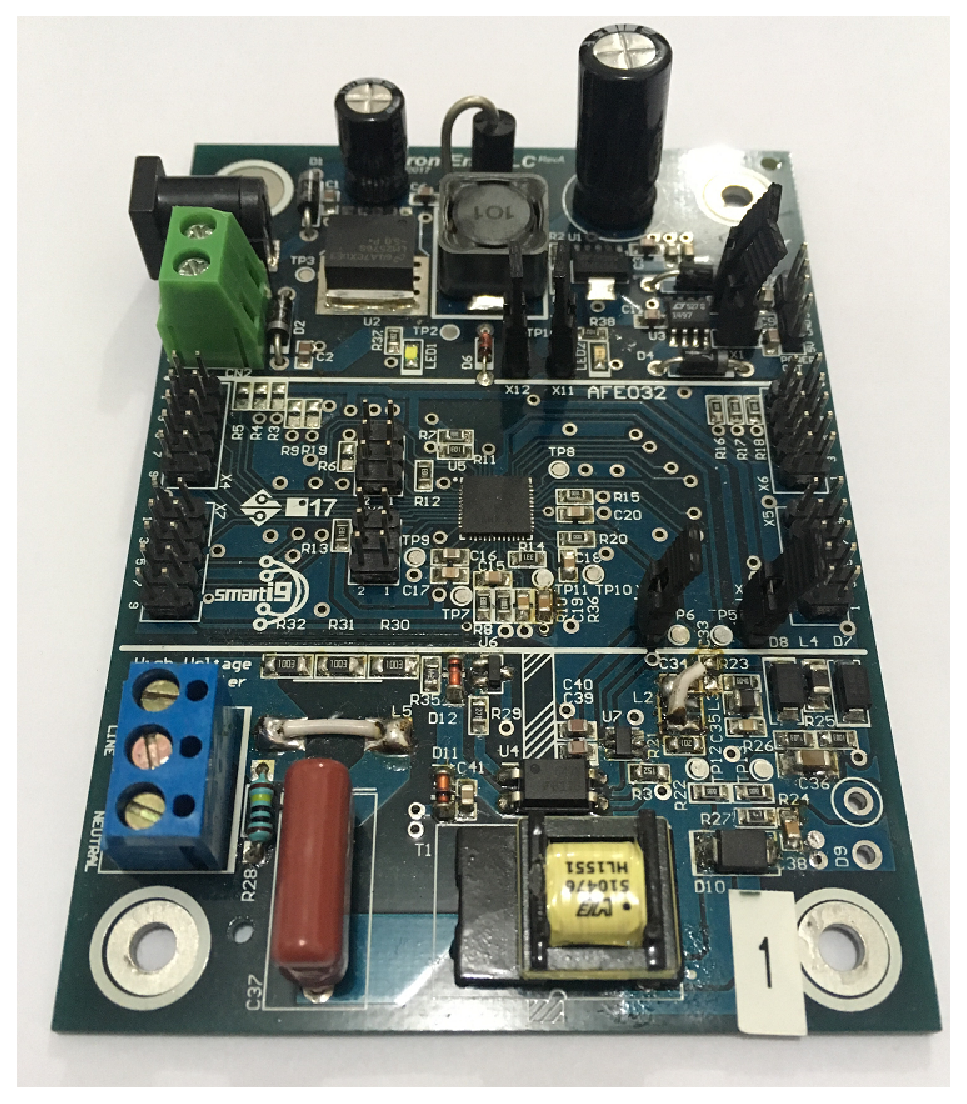
\includegraphics[width=0.45\linewidth]{figuras/AFE032}
		\caption{PLC analog front-end.}
		\label{fig:afe032}
	\end{figure}
\end{frame}

\begin{frame}
	\frametitle{\normalsize{Prototyping the NB hybrid PLC/Wireless transceiver}}
	\framesubtitle{The NB hybrid PLC/Wireless transceiver prototype}
	\begin{figure}[ht]
		\centering
		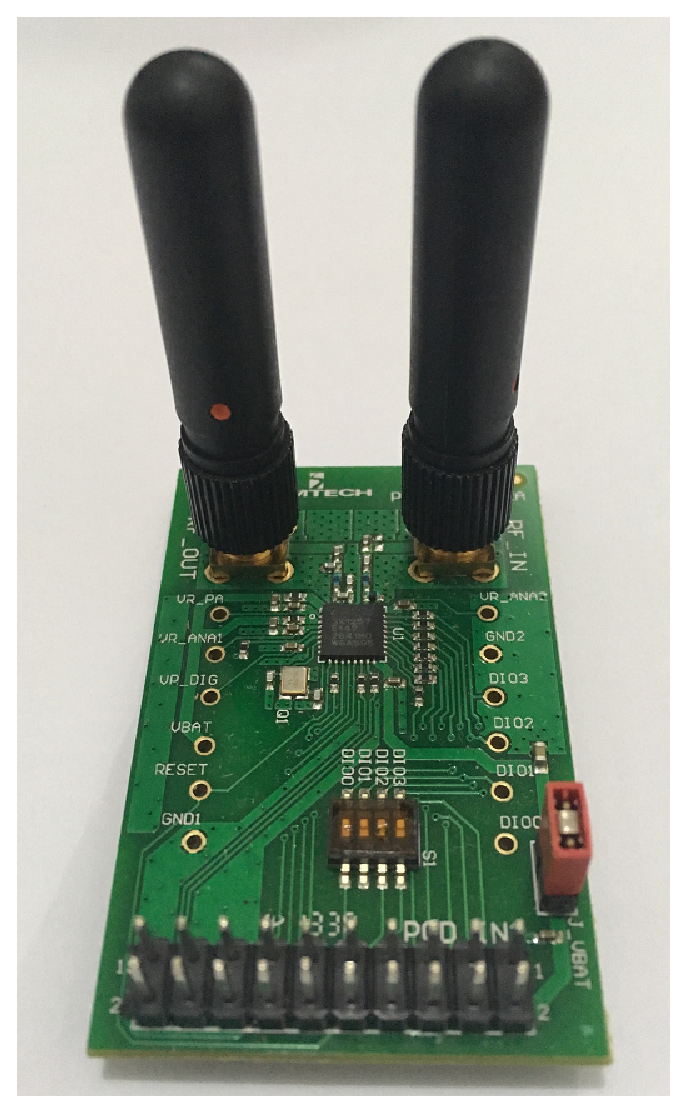
\includegraphics[width=0.30\linewidth]{figuras/SX1257}
		\caption{Wireless analog front-end.}
		\label{fig:sx1257}
	\end{figure}
\end{frame}

%------------------------------------------------------------------------------------
\section{Performance analyses}
\begin{frame}
	\frametitle{Outlines}
	\small
	\tableofcontents[currentsection]
\end{frame}
%------------------------------------------------------------------------------------
\subsection{Decision Maker time analysis}
%%-----------------------------------------------
\begin{frame}
	\frametitle{Performance analyses}
	\framesubtitle{Decision Maker time analysis}
	\begin{figure}[ht]
		\centering
		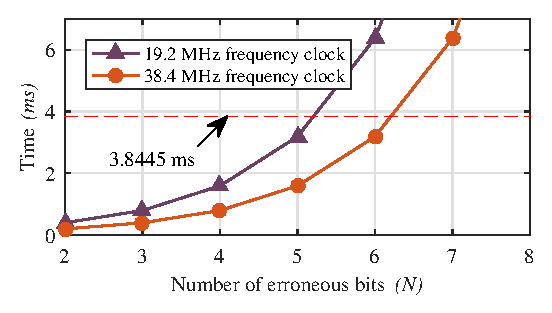
\includegraphics[width=0.9\linewidth]{figuras/decision_maker}
		\caption{Time interval demanded by the Decision Maker block.}
		\label{fig:decisionmaker}
	\end{figure}
\end{frame}

%%-----------------------------------------------
\subsection{Physical layer data-rate analysis}
%%-----------------------------------------------
\begin{frame}
\frametitle{Outlines}
\small
\tableofcontents[currentsubsection]
\end{frame}

\begin{frame}
	\frametitle{Performance analyses}
	\framesubtitle{Physical layer data-rate analysis}
	\begin{table}[ht]
		\centering
		\caption{Data-rates of the NB hybrid PLC/Wireless transceiver.}
		\label{tab:data_rate}
		\begin{tabular}{c|c}
			\hline
			Modulation 			& Data-rate (kbps)  \\ \hline\hline
			S-ROBO (BPSK)    	& 14.4182          	\\ \hline
			ROBO (BPSK)       	& 23.3236          	\\ \hline
			BPSK       			& 101.3517         	\\ \hline
			QPSK       			& 210.3366         	\\ \hline
			8-PSK       			& 318.8974         	\\ \hline
		\end{tabular}
	\end{table}
\end{frame}

%%-----------------------------------------------
\subsection{Hardware resource usage analysis}
%%-----------------------------------------------
\begin{frame}
\frametitle{Outlines}
\small
\tableofcontents[currentsubsection]
\end{frame}

\begin{frame}
\frametitle{Performance analyses}
\framesubtitle{Hardware resource usage analysis}
\begin{table}[h]
	\centering
	\caption{Hardware resource usage per block.}
	\label{tab:hrublock}
	\scalebox{0.6}{
	\begin{tabular}{c|c|c|c|c|c|c|c}
		\hline
		\multirow{2}{*}{Block} & \multicolumn{4}{c|}{LE}                                        & \multirow{2}{*}{Memory bits} & \multirow{2}{*}{M9Ks} & \multirow{2}{*}{DSP} \\ \cline{2-5}
		& LUT-Only LEs & Register-Only LEs & LUT/Register LEs & Total LE &                              &                       &                      \\ \hline\hline
		Hilbert transform      & 833          & 315               & 765              & \alert{1913}     & 60                   & 1                     & 0                    \\ \hline
		Synchronism            & 2971         & 671               & 1853             & 5495     & 290634                       & 52                    & \alert{27}                   \\ \hline
		RX IEEE 1901.2         & 7624         & 2792              & 7556             & \alert{17972}    & 146232                       & 55                    & 20                   \\ \hline
		TX IEEE 1901.2         & 4910         & 2007              & 5523             & \alert{12440}    & 676800                       & 114                   & 12                   \\ \hline
		Decision Maker         & 170          & 104               & 205              & 479      & 3968                         & 2                     & 0                    \\ \hline
		P-AFE                  & 88           & 84                & 154              & 326      & 0                            & 0                     & 0                    \\ \hline
		W-AFE                  & 232          & 82                & 275              & 589      & 0                            & 30                    & 0                    \\ \hline
		MAC sublayer           & 6140         & 2002              & 5778             & \alert{13920}    & 990726                       & 152                   & 29                   \\
		\hline
		Total available           & -         & -              & -             &  114480    & 3888000                       & 436                   & 266                   \\
		 \hline
	\end{tabular}
}
\end{table}
\end{frame}

\begin{frame}
	\frametitle{Performance analyses}
	\framesubtitle{Hardware resource usage analysis}
	\textbf{NB PLC transceiver:}
	\begin{itemize}
		\item MAC sublayer, Hilbert transform, synchronism block, PHY TX IEEE 1901.2, PHY RX IEEE 1901.2, and a P-AFE block. \wait
	\end{itemize}
	
	\textbf{NB hybrid PLC/Wireless transceiver:} 
	\begin{itemize}
		\item MAC sublayer, two Hilbert transforms, two synchronism blocks, PHY TX IEEE 1901.2, two PHY RX IEEE 1901.2, the Decision Maker block, P-AFE block, and W-AFE block. \wait
	\end{itemize}
\end{frame}

\begin{frame}
	\frametitle{Performance analyses}
	\framesubtitle{Hardware resource usage analysis}
	\begin{table}[ht]
		\centering
		\caption{Hardware resource usage for NB PLC and NB hybrid PLC/Wireless transceiver prototypes.}
		\label{tab:hru}	
		\begin{tabular}{c|c|c|c|c}
			\hline
			\multicolumn{2}{c|}{Hardware resource} & PLC     & PLC-Wireless & $\rho$ \\ \hline
			\multirow{4}{*}{LE} & LUT-Only LEs      & 22566   & 34396        & 0.524        \\ \cline{2-5} 
			& Register-Only LEs & 7871    & 11835        & 0.503        \\ \cline{2-5} 
			& LUT/Register LEs  & 21629   & 32283        & 0.492        \\ \cline{2-5} 
			& Total LE          & 52066   & 78514        & 0.508        \\ \hline
			\multicolumn{2}{c|}{Memory}            & 2104452 & 2545346      & 0.209        \\ \hline
			\multicolumn{2}{c|}{M9Ks}              & 374     & 514          & 0.374        \\ \hline			
			\multicolumn{2}{c|}{DSP}         & 88      & 135          & 0.534        \\ \hline
			\multicolumn{2}{c|}{$f_{\max}$ (MHz)}              & 19.68   & 19.67        & -0.005        \\ \hline
			\multicolumn{2}{c|}{Power consumption (mW)} & 311.92  & 348.4        & 0.117        \\ \hline		
		\end{tabular}
	\end{table}
\end{frame}

%------------------------------------------------------------------------------------
\section{Conclusions}
\begin{frame}
	\frametitle{Outlines}
	\small
	\tableofcontents[currentsection]
\end{frame}
%------------------------------------------------------------------------------------
\begin{frame}
	\frametitle{Conclusions}
	%\framesubtitle{}
	\begin{itemize}
		\item The best choice concerning the approach to be	adopted is to \textbf{use a PLC standard and extend it to be used in the wireless medium}. \wait
		\item The IEEE 1901.2 Standard showed up as the most \textbf{promising} standard. \wait
		\item The Hilbert transform allows the \textbf{estimation and correction of the frequency deviation} between the transmitter and receiver’s clock. \wait
		\item The routing between nodes \textbf{rises system coverage and reliability}. \wait
		\item Decision Maker block \textbf{reduces the necessity of ARQ messages} and, consequently, it increases the data network throughput.
	\end{itemize}
\end{frame}

\begin{frame}
\frametitle{Conclusions}
%\framesubtitle{}
\begin{itemize}
	\item  Regarding the Decision Maker block time analysis, \textbf{it is not worth rising the PHY layer clock frequency} in order to be able to correct a great number of bits. \wait
	\item  The data-rate varies from a \textbf{few tens} of kbps up to a \textbf{few hundred} of kbps. \wait
	\item NB hybrid PLC/Wireless transceiver \textbf{consumes less than twice} the hardware resource usage and power consumption of the NB PLC transceiver. \wait
	\item  It is an expected result, having in mind that the NB hybrid PLC/Wireless transceiver was	implemented \textbf{aiming to increase performance and save hardware resources}.
\end{itemize}
\end{frame}

\begin{frame}
\frametitle{Future works}
%\framesubtitle{}
\begin{itemize}
	\item  To test the NB hybrid PLC/Wireless transceiver prototype in the field, facing more	realistic and variety situations. \wait
%	\item  To verify under which channel conditions the Decision Maker block can provide a maximum and a minimum performance. \wait
	\item To improve AFE interface blocks, making them able to automatically reconfigure	the AFEs to adapt to current channel conditions. \wait
%	\item Study of the P-AFE and W-AFE’s behavior in several channel conditions.
\end{itemize}
\end{frame}

\begin{frame}
	\frametitle{Publications}
	\framesubtitle{List of journal and conference papers}
	The list of journal papers submitted during the graduate period is as follows:
	\small
	\begin{itemize}
		\item DA COSTA, VINÍCIUS LAGROTA R.; FERNANDES, VICTOR; RIBEIRO, MOISÉS VIDAL, "A Prototype of a Narrowband Hybrid PLC/Wireless Transceiver," \linebreak \textit{IEEE Internet of Things}, 2017, under review.
		\item COSTA, LUIS GUILHERME DA SILVA; COLEN, GUILHERME R., QUEIROZ, ANTÔNIO CARLOS MOREIRÃO DE; DA COSTA, VINÍCIUS LAGROTA R.; VÍTOR, ULYSSES R. C.; RIBEIRO, MOISÉS VIDAL. "Access Impedance in Brazilian In-Home Broadband and Low-voltage Electric Power Grids: Measurement, Characterization and Modeling," \textit{Journal of Communication and Information Systems (JCIS)},\textit{Electric Power Systems Research}, 2017, under review.	
	\end{itemize}

\end{frame}

\begin{frame}
\frametitle{Publications}
\framesubtitle{List of journal and conference papers}
	The list of journal papers submitted during the graduate period is as follows:
	\small
	\begin{itemize}
		\item DA COSTA, VINÍCIUS LAGROTA R.; SCHETTINO, HUGO VIVEIROS; CAMPONOGARA, ÂNDREI; DE CAMPOS, FABRÍCIO P.V.; RIBEIRO, MOISÉS VIDAL. "Digital filters for clustered-OFDM-based PLC systems: Design and implementation". \textit{Digital Signal Processing}, v. 70, p. 166-177, 2017.
		
		\item COSTA, LUIS GUILHERME DA SILVA; DE QUEIROZ, ANTÔNIO CARLOS MOREIRÃO; ADEBISI, BAMIDELE; DA COSTA, VINICIUS LAGROTA RODRIGUES; RIBEIRO, MOISÉS VIDAL. "Coupling for Power Line Communications: A Survey". \textit{Journal of Communication and Information Systems (JCIS)}, v. 32, p. 8-22, 2017.
	\end{itemize}	
\end{frame}

\begin{frame}
	\frametitle{Publications}
	\framesubtitle{List of journal and conference papers}
	The list of conference papers published during the graduate period is as follows (SBrT):
	\small
	\begin{itemize}
		\item COSTA, V. L. R.; MIRANDA, C. R.; SOUZA, S. A.; MARTINS, C. H. N.; CAMPOS, F. P. V.; OLIVEIRA, T. R.; RIBEIRO, M. V. "Front-End Analógico para Power Line Communication na faixa entre 1.7 e 50 MHz". In: \textit{XXXIII Simpósio Brasileiro de Telecomunicações}, 2015, Juiz de Fora. SBrT, 2015.
		
		\item COSTA, L. G. S.; PICORONE, A. A. M.; COSTA, V. L. R.; RIBEIRO, M. V. "Projeto e Caracterização de Acopladores para Power Line Communication". In: \textit{XXXIII Simpósio Brasileiro de Telecomunicações}, 2015, Juiz de Fora. SBrT, 2015.
		
		\item COSTA, L. G. S.; PICORONE, A. A. M.; QUEIROZ, A. C. M.; COSTA, V. L. R.; RIBEIRO, M. V. "Caracterização da Impedância de Acesso à Rede de Energia Elétrica Residencial para Uso em Sistemas Power Line Communications". In: \textit{XXXIII Simpósio Brasileiro de Telecomunicações}, 2015, Juiz de Fora. SBrT, 2015.
	\end{itemize}
\end{frame}


%------------------------------------------------
\begin{frame}[noframenumbering]
	\vfill
	\centering
	\Huge{Thank you!}
	\vfill
\end{frame}

\end{document}
